

\chapter{Test Bench Part 2}

\section{Introduction}

This chapter revisit the concept of testbench in \verb|HLS|, taking into account sequential desing and single cycle desing technique (\autoref{chap:single_desing_flow}). This concept has been seen before in \autoref{chap:testbench_sim_part_1} .\\

\todo{intro testbench part 2} \uti{intro testbench part 2:}

\begin{itemize}

\item \textit{To rewrite the introduction later when revisiting back the reader}

\end{itemize}


\newpage
\section{Testbench and Simulation Concept}

One of the verification technique in order to validate our desing is through \textit{simulation}, which can be separated into 2 part as shown in \autoref{fig:testbench_2:sim_test_intro}:

\begin{figure}[h]
\centering
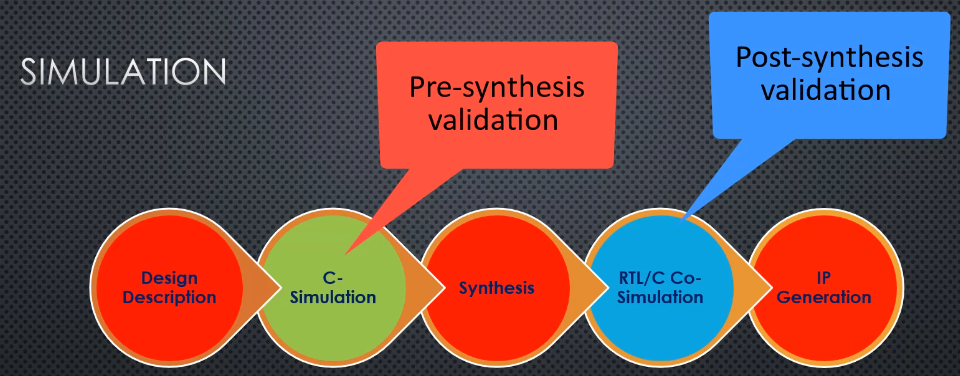
\includegraphics[scale=0.4,frame]{Figures/testbench_2/sim_test_intro}
\caption{Testbench and Simulation}
\label{fig:testbench_2:sim_test_intro}
\end{figure}

\begin{enumerate}

\item Presynthesis validation: checks if the \verb|C++| code correctly implement the functionality

	\begin{itemize}
	\item This step is done after implementing our \verb|HLS| code, that is the top level function, and before the synthesis 
	
	\item In \verb|Vitis|, this is done using \verb|C simulation| option under the flow navigator	
	
	\end{itemize}

\item Post synthesis validation: checks if the generated \verb|RTL| code behaves as expected

	\begin{itemize}
	\item This step is done after synthesis and before exporting the \verb|IP|
	
	
	\item In \verb|Vitis|, this is done via the option \verb|C-RTL cosimulation|
	\end{itemize}

\end{enumerate}


In \autoref{chap:single_desing_flow}, we learned the single cycle desing flow, so now we will adjust \verb|C simulation| for the parallel-serial system, to validate the desing cycle by cycle.\\

In a more general way, when performing testbench throughout \verb|C simulation|, we don't have any knowledge about timing, so now we take timing into consideration.


\uti{C sim and timing} \todo{C sim and timing}

\begin{itemize}

\item \textit{After finishing the chapter, I need to understand what is the meaning of the paragprah above}

	\begin{itemize}
	\item \textit{Is it like we are testing timing or validating some timing constraint ?}
	
	\item \textit{To see after}	
	
	\end{itemize}

\end{itemize}


\uti{Merge testbench part 2:} \todo{Merge testbench part 2}

\begin{itemize}

\item \textit{Maybe after I will merge this chapter with \autoref{chap:single_desing_flow} }

\end{itemize}

\subsection{Quiz}

\underline{Given:} what are the benefits of single desing over multi-cycle desing approach ?

\underline{Solution:}

\begin{enumerate}

\item The circuit can receive data in each clock cycle and can increase the
circuit performance if the circuit can accept the maximum clock
frequency available for the FPGA

\item The circuit can generate output in each clock cycle which can provide
high throughput

\item Potentially it can reduce the handshaking during communication with
other single-cycle modules
 
\end{enumerate}








 







